\chapter{Evaluation}\label{chap:evaluation}

This section reflects the results of all the testing performed with the different programming languages and architectures / types of computer.

\begin{table}[ht]
  \centering
  \begin{tabular}{lcccc}
    \toprule
                            & C\++                  & Go        & Python        & PyPy \\
    \midrule
    Intel Xeon Gold 6326 x2 &  GCC 14.2.0           & go1.24.2  & Python 3.12.3 & PyPy 7.3.19 \\
    MacbookPro M4 Pro       &  Apple Clang 17.0.0   & go1.24.2  & Python 3.13.3 & PyPy 7.3.19 \\
    RPi 5                   &                       &           &               &             \\
    Ryzen 3800x             &                       &           &               &             \\
    \bottomrule
  \end{tabular}
  \caption{Comparison of language performance on different platforms}
  \label{tab:lang-platforms}
\end{table}

It should be noted that python should not be used for performance critical applications, as it is an interpreted language, and it is not designed for high performance computing. However, it is a great language for rapid prototyping and development, and it is widely used in the industry. 

Go's intent is to be a fast, efficient, and easy to use language, and it is designed for multithreading and concurrency, which makes it a great choice for high performance computing, specifically being designed for backend development for web applications, and it is widely used in the industry.

\section{Measurement Platforms}
\subsection{Many Core Platform}

This platform is the most powerful combinations as well as power-hungry combinations of all of my suite of devices. This is a rack server, with two processors Intel Xeon Gold 6326, that have each 16 cores, 32 threads, contributing to a total of 32 cores, 64 threads. It also has the largest amount of \gls{ram} from this testing, with 256GB of \gls{DDR4} memory.

As it has two sockets, one per CPU chip, there has to be an intercommunication between these processors if a process spreads out to more than 32 threads, or is set by the user using the command \texttt{taskset}, fixing the cores the process can run on.



%% Comments on the platform, ie two xeon 16 cores processors with hyperthreading, x86
\subsubsection{Evaluated parameters}
This system was the most versatile in terms of how many  tests could be done, as it has many processors, and uses Linux on X86, a great advantage to force processes to run on specific cores

The tests were done on a variety of core configuration, always setting, for core numbers less than 16, cores in the same processor. 

\begin{itemize}
    \item \textbf{1 Core}: Testing with one core, producing the baseline for the programs energy consumption and time.
    \item \textbf{2 Cores}: Testing with 2 cores provides the first glimpse of parallelization.
    \item \textbf{4 Cores}: Testing with 4 cores because many computer from some time ago had for cores.
    \item \textbf{8 Cores}: Testing with 8 cores gives us a great insight into how many processors in the market work, and it is half of the amount of cores inside one chip.
    \item \textbf{14 Cores}: Testing with 14 cores, because it is the number of cores available on the Laptop and wanted to have an execution time comparison. 
    \item \textbf{16 Cores}: Testing with 16 cores as it is the amount or real cores on a single chip. This must be one of the most energy efficient and fast tests, if there were only one \gls{cpu}.
    \item \textbf{28 Cores (in different \glspl{cpu}, but all real cores, no logical cores)}: Testing with 28 cores, distributed with two sockets is interesting because there has to be some information sharing over some bun inside the motherboard to synchronize both \glspl{cpu}. This wont be as energy efficient, but may be faster.
    \item \textbf{28 Cores (in the same CPU, 16 cores, 32 virtual cores)}: Testing with 28 cores, inside the same CPU, the performance should be slower as there are less real cores to tackle the work, but it has the advantage of not needing to share data to another socket.
    \item \textbf{32 Cores (same socket)}: Testing with 32 cores in the same socket is using all available logical threads of a system, the 16 real cores and the other 16 threads the \gls{cpu} has thanks to Hyper-Threading.
    \item \textbf{32 Cores (only real cores)}: Testing with 32 real cores, across two sockets should be the most powerful combination for CPU intensive tasks, as all the operations should be able to be carried out without many interruptions.
    \item \textbf{48 Cores}: Testing with 48 cores forces us to use all real cores and some logical cores.
    \item \textbf{60 Cores}: Testing with 60 cores is also interesting and not 64, as this would force the machine to interrupt the program we are benchmarking to perform routine operations, such as checking for incoming connections, or logging.
\end{itemize}

\subsubsection{Results}

The results for the server are shown in the following figures and tables. The energy consumption is measured in joules, and the execution time is measured in seconds. 

\begin{figure}[H]
  \centering
  \begin{tikzpicture}
  \begin{semilogyaxis}[
      title={Logarithmic energy (pkg) consumption - Server},
      width=\plotwidthgraph,
      height=\plotheightgraph,
      xlabel={Number of Cores},
      ylabel={Energy (J)},
      ymode=log,
      xmode=linear,
      grid=both,
      minor tick num=1,
      grid style={gray!30,dashed},
      xtick={1,2,4,8,14,16,28,32,48,60},
      x tick label style={
        font=\footnotesize,
        rotate=45,
        anchor=north east
      },
      legend style={
        at={(0.98,0.98)},
        anchor=north east,
        font=\scriptsize,
        nodes={scale=0.8,transform shape},
        draw=none
      },
      legend columns=2,
      transpose legend,
      legend cell align=left,
    ]

    %% C++ %%
    % open circles
    \addplot[
      blue,
      only marks,
      mark=o,
      mark options={draw=blue,fill=white}
    ] table[row sep=\\] {
      x    y \\
      1    3756.26  \\
      2    2591.91  \\
      4    1362.61  \\
      8    799.23   \\
      14   603.37   \\
      16   627.16   \\
      28   541.37   \\  
      32   529.61   \\  
      48   740.57   \\
      60   666.04   \\
    };
    \addlegendentry{C++}
    % filled circles at 28 & 32
    \addplot[
      blue,
      only marks,
      mark=*,
      mark options={draw=blue,fill=blue}
    ] table[row sep=\\] {
      x    y \\
      28   766.51   \\  
      32   757.79   \\  
    };
    \addlegendentry{C++ same CPU}
    % trendline, but do NOT add to legend:
    \addplot[
      blue,
      dashed,
      forget plot,
      domain=1:60,
      samples=200
    ] {3000 * x^(-0.4513)};

    %% Go %%
    \addplot[
      violet,
      only marks,
      mark=o,
      mark options={draw=violet,fill=white}
    ] table[row sep=\\] {
      x    y \\
      1    28522.69 \\
      2    18231.97 \\
      4    10304.27	\\
      8    5617.27  \\
      14   3155.30  \\
      16   2904.52  \\
      28   2306.35  \\
      32   2151.74  \\
      48   1856.93  \\
      60   1744.76  \\
    };
    \addlegendentry{Go}
    \addplot[
      violet,
      only marks,
      mark=*,
      mark options={draw=violet,fill=violet}
    ] table[row sep=\\] {
      x    y \\
      28   2271.71  \\
      32   2109.37  \\
    };
    \addlegendentry{Go same CPU}
    \addplot[
      violet,
      dashed,
      forget plot,
      domain=1:60,
      samples=200
    ] {23600 * x^(-0.6783)};

    %% PyPy %%
    \addplot[
      orange,
      only marks,
      mark=o,
      mark options={draw=orange,fill=white}
    ] table[row sep=\\] {
      x    y \\
      1    7972.65  \\
      2    5147.60  \\
      4    2828.21  \\
      8    1747.96  \\
      14   1232.03  \\
      16   1140.80  \\
      28   1252.93  \\
      32   1257.81  \\
      48   1354.03  \\
      60   1354.03  \\
    };
    \addlegendentry{PyPy}
    \addplot[
      orange,
      only marks,
      mark=*,
      mark options={draw=orange,fill=orange}
    ] table[row sep=\\] {
      x    y \\
      28   1175.52  \\
      32   1155.74  \\
    };
    \addlegendentry{PyPy same CPU}
    \addplot[
      orange,
      dashed,
      forget plot,
      domain=1:60,
      samples=200
    ] {6250 * x^(-0.4633)};

    %% Python %%
    \addplot[
      green!60!black,
      only marks,
      mark=o,
      mark options={draw=green!60!black,fill=white}
    ] table[row sep=\\] {
      x    y \\
      1    1510534.76 \\
      2    1141490.15 \\
      4    313537.85  \\
      8    194458.98  \\
      14   130506.94  \\
      16   111438.01  \\
      28   122384.40  \\
      32   120259.78  \\
      48   97331.00   \\
      60   93718.97   \\
    };
    \addlegendentry{Python}
    \addplot[
      green!60!black,
      only marks,
      mark=*,
      mark options={draw=green!60!black,fill=green!60!black}
    ] table[row sep=\\] {
      x    y \\
      28   96049.86 \\  
      32   87343.61 \\
    };
    \addlegendentry{Python same CPU}
    \addplot[
      green!60!black,
      dashed,
      forget plot,
      domain=1:60,
      samples=200
    ] {1.27e6 * x^(-0.7046)};

  \end{semilogyaxis}
\end{tikzpicture}
\caption{Server - Logarithmic energy (pkg) consumption}{Logarithm energy (pkg) consumption of the Server benchmark across different programming languages.}
\label{fig:log-server-energy-pkg}
\end{figure}


\begin{figure}[h]
  \centering
  \begin{tikzpicture}
  \begin{axis}[
      title={Energy efficiency speedup},
      width=\plotwidthgraph,
      height=\plotheightgraph,
      xlabel={Number of Cores},
      ylabel={Speedup (relative to 1 core)},
      xmode=linear,
      grid=both,
      minor tick num=1,
      grid style={gray!30,dashed},
      xtick={1,2,4,8,14,16,28,32,48,60},
      x tick label style={
        font=\footnotesize,
        rotate=45,
        anchor=north east
      },
      legend style={
        at={(0.02,0.98)},
        anchor=north west,
        font=\scriptsize,
        nodes={scale=0.8,transform shape},
        draw=none
      },
      legend columns=1,
      legend cell align=left,
      ymin=0,
      ymax=18,
    ]

    %% C++ Speedup (Energy efficiency improvement) %%
    \addplot[
      blue,
      mark=o,
      mark options={draw=blue,fill=white},
      line width=1.5pt
    ] table[row sep=\\] {
      x    y \\
      1    1.00  \\
      2    1.45  \\
      4    2.76  \\
      8    4.70  \\
      14   6.22  \\
      16   5.99  \\
      28   6.94  \\  
      32   7.09  \\  
      48   5.07  \\
      60   5.64  \\
    };
    \addlegendentry{C++}
    
    \addplot[
      blue,
      only marks,
      mark=*,
      mark options={draw=blue,fill=blue}
    ] table[row sep=\\] {
      x    y \\
      28   4.90  \\  
      32   4.95  \\  
    };
    \addlegendentry{C++ same CPU}

    %% Go Speedup %%
    \addplot[
      violet,
      mark=o,
      mark options={draw=violet,fill=white},
      line width=1.5pt
    ] table[row sep=\\] {
      x    y \\
      1    1.00  \\
      2    1.56  \\
      4    2.77  \\
      8    5.08  \\
      14   9.04  \\
      16   9.82  \\
      28   12.37 \\
      32   13.26 \\
      48   15.36 \\
      60   16.35 \\
    };
    \addlegendentry{Go}
    
    \addplot[
      violet,
      only marks,
      mark=*,
      mark options={draw=violet,fill=violet}
    ] table[row sep=\\] {
      x    y \\
      28   12.56 \\
      32   13.52 \\
    };
    \addlegendentry{Go same CPU}

    %% PyPy Speedup %%
    \addplot[
      orange,
      mark=o,
      mark options={draw=orange,fill=white},
      line width=1.5pt
    ] table[row sep=\\] {
      x    y \\
      1    1.00  \\
      2    1.55  \\
      4    2.82  \\
      8    4.56  \\
      14   6.47  \\
      16   6.99  \\
      28   6.36  \\
      32   6.34  \\
      48   5.89  \\
      60   5.89  \\
    };
    \addlegendentry{PyPy}
    
    \addplot[
      orange,
      only marks,
      mark=*,
      mark options={draw=orange,fill=orange}
    ] table[row sep=\\] {
      x    y \\
      28   6.78  \\
      32   6.90  \\
    };
    \addlegendentry{PyPy same CPU}

    %% Python Speedup %%
    \addplot[
      green!60!black,
      mark=o,
      mark options={draw=green!60!black,fill=white},
      line width=1.5pt
    ] table[row sep=\\] {
      x    y \\
      1    1.00  \\
      2    1.32  \\
      4    4.82  \\
      8    7.77  \\
      14   11.57 \\
      16   13.55 \\
      28   12.34 \\
      32   12.56 \\
      48   15.52 \\
      60   16.11 \\
    };
    \addlegendentry{Python}
    
    \addplot[
      green!60!black,
      only marks,
      mark=*,
      mark options={draw=green!60!black,fill=green!60!black}
    ] table[row sep=\\] {
      x    y \\
      28   15.73 \\  
      32   17.29 \\
    };
    \addlegendentry{Python same CPU}

  \end{axis}
  \end{tikzpicture}
\caption{Server - Speedup Energy Efficiency}{Server benchmark energy performance comparison across programming languages: Energy efficiency speedup relative to single-core performance (higher is better).}
\label{fig:energy-comparison}
\end{figure}


\begin{figure}
  \centering
  \begin{tikzpicture}
  \begin{semilogyaxis}[
      title={Logarithmic energy (ram) consumption - Server},
      width=\plotwidthgraph,
      height=\plotheightgraph,
      xlabel={Number of Cores},
      ylabel={Energy (J)},
      ymode=log,
      xmode=linear,
      grid=both,
      minor tick num=1,
      grid style={gray!30,dashed},
      xtick={1,2,4,8,14,16,28,32,48,60},
      x tick label style={
        font=\footnotesize,
        rotate=45,
        anchor=north east
      },
      legend style={
        at={(0.98,0.98)},
        anchor=north east,
        font=\scriptsize,
        nodes={scale=0.8,transform shape},
        draw=none
      },
      legend columns=2,
      transpose legend,
      legend cell align=left,
    ]

    %% C++ %%
    \addplot[
      blue,
      only marks,
      mark=o,
      mark options={draw=blue,fill=white}
    ] table[row sep=\\] {
      x    y \\
      1    176.83  \\
      2    111.08  \\
      4    67.60   \\
      8    26.28   \\
      14   18.28   \\
      16   19.29   \\
      28   16.91   \\
      32   17.80   \\
      48   27.02   \\
      60   24.40   \\
    };
    \addlegendentry{C++}
    \addplot[
      blue,
      only marks,
      mark=*,
      mark options={draw=blue,fill=blue}
    ] table[row sep=\\] {
      x    y \\
      28   29.01   \\
      32   28.15   \\
    };
    \addlegendentry{C++ same CPU}
    % power‐law fit: y = 138.9 * x^(–0.5506)
    \addplot[
      blue,
      forget plot,
      domain=1:60,
      samples=200
    ] {128.71 * x^(-0.540)};

    %% Go %%
    \addplot[
      violet,
      only marks,
      mark=o,
      mark options={draw=violet,fill=white}
    ] table[row sep=\\] {
      x    y \\
      1    1049.92 \\
      2    755.43  \\
      4    426.69  \\
      8    175.15  \\
      14   107.26  \\
      16   95.60   \\
      28   55.09   \\
      32   61.70   \\
      48   85.73   \\
      60   90.01   \\
    };
    \addlegendentry{Go}
    \addplot[
      violet,
      only marks,
      mark=*,
      mark options={draw=violet,fill=violet}
    ] table[row sep=\\] {
      x    y \\
      28   78.01   \\
      32   65.66   \\
    };
    \addlegendentry{Go same CPU}
    % power‐law fit: y = 1024.9 * x^(–0.7437)
    \addplot[
      violet,
      forget plot,
      domain=1:60,
      samples=200
    ] {975.38 * x^(-0.728)};

    %% PyPy %%
    \addplot[
      orange,
      only marks,
      mark=o,
      mark options={draw=orange,fill=white}
    ] table[row sep=\\] {
      x    y \\
      1    355.42  \\
      2    253.06  \\
      4    170.08  \\
      8    88.94   \\
      14   72.28   \\
      16   71.84   \\
      28   81.44   \\
      32   83.50   \\
      48   89.06   \\
      60   91.31   \\
    };
    \addlegendentry{PyPy}
    \addplot[
      orange,
      only marks,
      mark=*,
      mark options={draw=orange,fill=orange}
    ] table[row sep=\\] {
      x    y \\
      28   78.81   \\
      32   77.79   \\
    };
    \addlegendentry{PyPy same CPU}
    % power‐law fit: y = 292.4 * x^(–0.3661)
    \addplot[
      orange,
      forget plot,
      domain=1:60,
      samples=200
    ] {273.36 * x^(-0.357)};

    %% Python %%
    \addplot[
      green!60!black,
      only marks,
      mark=o,
      mark options={draw=green!60!black,fill=white}
    ] table[row sep=\\] {
      x    y \\
      1    59269.48 \\
      2    36442.43 \\
      4    12799.44 \\
      8    6683.08  \\
      14   4031.07  \\
      16   3705.32  \\
      28   4057.46  \\
      32   4037.98  \\
      48   2850.62  \\
      60   2703.02  \\
    };
    \addlegendentry{Python}
    \addplot[
      green!60!black,
      only marks,
      mark=*,
      mark options={draw=green!60!black,fill=green!60!black}
    ] table[row sep=\\] {
      x    y \\
      28   2831.52 \\
      32   2576.33 \\
    };
    \addlegendentry{Python same CPU}
    % power‐law fit: y = 4.79e4 * x^(–0.7649)
    \addplot[
      green!60!black,
      forget plot,
      domain=1:60,
      samples=200
    ] {45451.50 * x^(-0.760)};

  \end{semilogyaxis}
\end{tikzpicture}
\caption{Server - Logarithmic energy (ram) consumption}{Logarithm energy (ram) consumption of the Server benchmark across different programming languages.}
\label{fig:log-server-energy-ram}
\end{figure}




\begin{figure}
  \centering

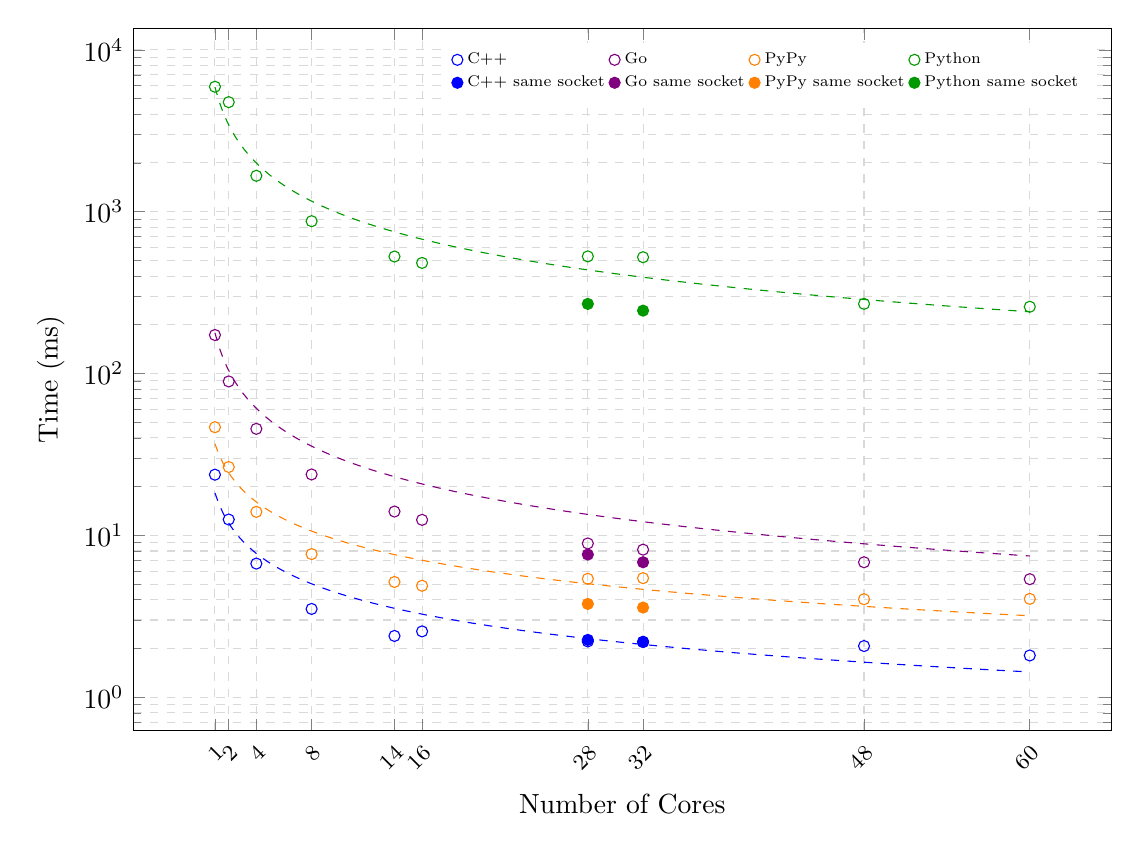
\begin{tikzpicture}
  \begin{semilogyaxis}[
      width=14cm,
      height=10.5cm,
      xlabel={Number of Cores},
      ylabel={Time (ms)},
      ymode=log,
      xmode=linear,
      grid=both,
      minor tick num=1,
      grid style={gray!30,dashed},
      xtick={1,2,4,8,14,16,28,32,48,60},
      x tick label style={
        font=\footnotesize,
        rotate=45,
        anchor=north east
      },
      legend style={
        at={(0.98,0.98)},
        anchor=north east,
        font=\scriptsize,
        nodes={scale=0.8,transform shape},
        draw=none
      },
      legend columns=2,
      transpose legend,
      legend cell align=left,
    ]

    %% C++ %%
    \addplot[
      blue,
      only marks,
      mark=o,
      mark options={draw=blue,fill=white}
    ]
    table[row sep=\\] {
      x    y \\
      1    23.70  \\
      2    12.52  \\
      4    6.69   \\
      8    3.51   \\
      14   2.39   \\
      16   2.55   \\
      28   2.21   \\
      32   2.20   \\
      48   2.07   \\
      60   1.81   \\
    };
    \addlegendentry{C++}

    \addplot[
      blue,
      only marks,
      mark=*,
      mark options={draw=blue,fill=blue}
    ]
    table[row sep=\\] {
      x    y \\
      28   2.26   \\
      32   2.19   \\
    };
    \addlegendentry{C++ same socket}

    % power‐law fit: y = 18.3 * x^(-0.6223)
    \addplot[
      blue,
      dashed,
      forget plot,
      domain=1:60,
      samples=200
    ] {18.3 * x^(-0.6223)};

    %% Go %%
    \addplot[
      violet,
      only marks,
      mark=o,
      mark options={draw=violet,fill=white}
    ]
    table[row sep=\\] {
      x    y \\
      1    172.952 \\
      2    89.32  \\
      4    45.51  \\
      8    23.78  \\
      14   14.03  \\
      16   12.46  \\
      28   8.91   \\
      32   8.16   \\
      48   6.82   \\
      60   5.36   \\
    };
    \addlegendentry{Go}

    \addplot[
      violet,
      only marks,
      mark=*,
      mark options={draw=violet,fill=violet}
    ]
    table[row sep=\\] {
      x    y \\
      28   7.61  \\
      32   6.82  \\
    };
    \addlegendentry{Go same socket}

    % power‐law fit: y = 178.3 * x^(-0.7753)
    \addplot[
      violet,
      dashed,
      forget plot,
      domain=1:60,
      samples=200
    ] {178.3 * x^(-0.7753)};

    %% PyPy %%
    \addplot[
      orange,
      only marks,
      mark=o,
      mark options={draw=orange,fill=white}
    ]
    table[row sep=\\] {
      x    y \\
      1    46.58  \\
      2    26.43  \\
      4    13.97  \\
      8    7.66   \\
      14   5.15   \\
      16   4.88   \\
      28   5.39   \\
      32   5.44   \\
      48   4.03   \\
      60   4.05   \\
    };
    \addlegendentry{PyPy}

    \addplot[
      orange,
      only marks,
      mark=*,
      mark options={draw=orange,fill=orange}
    ]
    table[row sep=\\] {
      x    y \\
      28   3.77   \\
      32   3.58   \\
    };
    \addlegendentry{PyPy same socket}

    % power‐law fit: y = 36.8 * x^(-0.5976)
    \addplot[
      orange,
      dashed,
      forget plot,
      domain=1:60,
      samples=200
    ] {36.8 * x^(-0.5976)};

    %% Python %%
    \addplot[
      green!60!black,
      only marks,
      mark=o,
      mark options={draw=green!60!black,fill=white}
    ]
    table[row sep=\\] {
      x    y \\
      1    5913.41  \\
      2    4749.55  \\
      4    1665.41  \\
      8    872.89   \\
      14   528.12   \\
      16   482.30   \\
      28   529.22   \\
      32   523.04   \\
      48   269.41   \\
      60   258.44   \\
    };
    \addlegendentry{Python}

    \addplot[
      green!60!black,
      only marks,
      mark=*,
      mark options={draw=green!60!black,fill=green!60!black}
    ]
    table[row sep=\\] {
      x    y \\
      28   269.13  \\
      32   244.57  \\
    };
    \addlegendentry{Python same socket}

    % power‐law fit: y = 5894 * x^(-0.7811)
    \addplot[
      green!60!black,
      dashed,
      forget plot,
      domain=1:60,
      samples=200
    ] {5894 * x^(-0.7811)};

  \end{semilogyaxis}
\end{tikzpicture}

\caption{Execution time of the server in Joules for different core configurations}
  \label{fig:server-execution-time}
\end{figure}

\begin{table}[ht]
    \centering
    \begin{tabular}{lrrrr}
        \hline
        time         & C++             & Go            & PyPy          & Python     \\
        \hline
        1            & 23.70           & 172.952       & 46.58         & 5,913.41        \\
        2            & 12.52           & 89.32         & 26.43         & 4,749.55        \\
        4            & 6.69            & 45.51         & 13.97         & 1,665.41        \\
        8	           & 3.51  	         & 23.78 	       & 7.66          & 872.89          \\
        14           & 2.39            & 14.03         & 5.15          & 528.12          \\
        16           & 2.55            & 12.46         & 4.88          & 482.30          \\
        28           & 2.21            & 8.91          & 5.39          & 529.22          \\
        28 same CPU  & 2.26            & 7.61          & 3.77          & 269.13          \\
        32           & 2.20            & 8.16          & 5.44          & 523.04          \\
        32 same CPU  & 2.19            & 6.82          & 3.58          & \textbf{244.57} \\
        48           & 2.07            & 6.82          & 4.03          & 269.41          \\
        60           & \textbf{1.81}   & \textbf{5.36} & \textbf{4.05} & 258.44          \\
        \hline
    \end{tabular}
    \caption{Execution time by implementation and core count}
    \label{tab:server-execution-time}
\end{table}



From \autoref{fig:server-energy-pkg} we can see that the energy consumption of the server is not linear with the number of cores. It can be observed that the energy consumption decreases as the number of cores increases, but there is a point in the graph and \autoref{tab:server-energy-pkg} where the energy consumption starts to increase slightly again, as well as the execution times in \autoref{fig:server-execution-time}, but not as much as the energy consumption. 
This is due to hyperthreading \footnote{Hyperthreading is enabled in this system as it it not mine and I can not dissable it to perform testing. To set the process to a fixed \gls{cpu}, I used \texttt{taskset -c [cores]} ie \texttt{taskset -c 0-15,32-47} for running across multiple \glspl{cpu} and \texttt{taskset -c 0-31} to force the prorgam to only run in a single \gls{cpu}} in the \glspl{cpu}, which allows the \glspl{cpu} to run two threads per core, but this is not as efficient as running a single thread per core, as the \glspl{cpu} have to share resources between the two threads.

It is obvious from the multiple graphs and tables that the C\++ implementation is the most energy efficient and fastest by a significant margin, followed suprsingly by the PyPy execution of the Python code, which is faster than the Go implementation, and the Python implementation is the slowest and most energy consuming by an extremely large amount.

I want to specifically talk about the 60 cores test, as it is the most interesting one. In this test, the energy consumption is lower than in the 48 cores test, as well as the execution time on the C++ implementation, but on the Go implementation, both energy consumption and execution time are higher than in the 48 cores test. This is because the Go implementation is not as efficient as the C\++ implementation, and the Go runtime has to manage more goroutines, which adds overhead. 

Considering the 32 and 48 cores tests with the python program, the energy consumption reduces significanly when the program start using virtual cores, as the program is able to run on more cores, and the python runtime is not very demanding, being able to use these cores efficiently, as shown in \autoref{fig:server-energy-pkg} and \autoref{fig:server-execution-time} is an advantage to python with respect to itself.



\begin{figure}
    \centering
    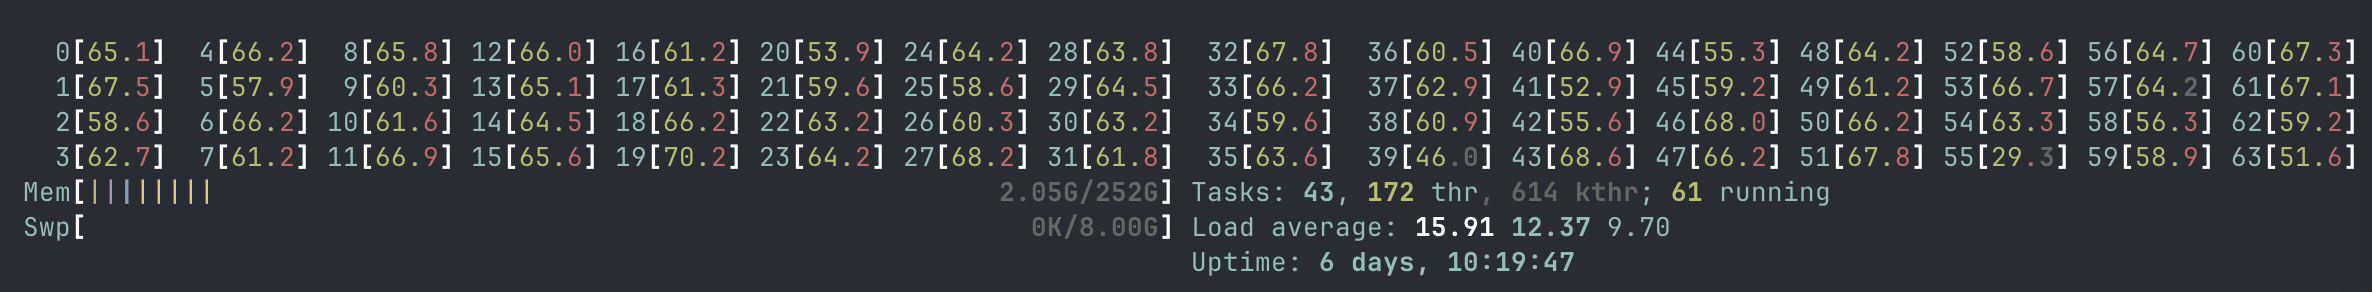
\includegraphics[width=1\linewidth]{img/htop_not_running_100_60_cores.png}
    \caption{Htop showing the cores not being used at 100\% when using many cores for processing in a per-pixel multi threading renderer }
    \label{fig:htop_60_not_100}
\end{figure}

It also must be noted that the cores during the 48 core benchmark were being used at 100\% of their capacity, while in the 60 cores test, the cores were mostly being usead at a lower percentage, as shown in \autoref{fig:htop_60_not_100}. This is because the Go runtime is not able to efficiently use all the cores when there are more than 48 cores available, and it is not able to schedule the goroutines efficiently as these routines finish so fast that the Go runtime is not able to keep all the cores busy.

If we changed the implementation to a per-row renderer, on the go-side, the Go runtime would be able to use all the cores more efficiently, as it would be able to schedule the goroutines more efficiently, and the execution time would be lower, but the energy consumption would be higher, as the cores would be used at 100\% of their capacity. Thus, in this case, as we will see in other sections, having a faster execution time is not always the best option in terms of energy consumption.




% When changin to a per-pixel rendered, lower cores energy efficiency increased, but the many cores, from 48 oward would not get used as much, thus reducing the energy efficiency and increating the execution time. 



\subsection{Personal Desktop}
%% Comments on the platform, ARM 14 core, big.LITTLE architecture (firestorm, 10 high performance cores and icestorm, 4 high efficiency cores)
\subsubsection{Evaluated parameters}
\subsubsection{Results}

\subsection{Personal SOTA Laptop}
%% Comments on the platform X86, 8 cores, 16 threads, AMR ZEN 2 (https://www.amd.com/en/support/downloads/drivers.html/processors/ryzen/ryzen-3000-series/amd-ryzen-7-3800x.html#amd_support_product_spec)
%% Test with and without hyerthreading as math intensive calculations
\subsubsection{Evaluated parameters}
\subsubsection{Results}

\subsection{Raspberry Pi 5}
\subsubsection{Evaluated parameters}
\subsubsection{Results}


\section{Comment on paralellizing different languages}

%% more threads than avaiable, is it beneficial?

%% Python
%% Why the multi-threaded version is slower iterating though every pixel:
%% Process creation overhead: The code uses ProcessPoolExecutor which creates separate Python processes for each pixel. Creating processes is much more expensive than creating threads, and doing it for every single pixel creates massive overhead.

%% Data serialization: Each time a task is submitted to a process, Python needs to serialize (pickle) the entire world object and other parameters, then deserialize them in the worker process. This happens for every pixel!

%% Too much granularity: Processing individual pixels in separate processes is extremely fine-grained parallelization. The overhead of process management far exceeds the actual computation time per pixel.

%% Memory overhead: Each process has its own memory space, so the world object is duplicated across all worker processes.